\documentclass[14pt,aspectratio=169]{beamer}
\setbeamertemplate{caption}[numbered]
\setbeamertemplate{caption label separator}{:}
\setbeamercolor{caption name}{fg=normal text.fg}
\usepackage{amssymb,amsmath}
\usepackage{ifxetex,ifluatex}
\usepackage{fixltx2e} % provides \textsubscript
\usepackage{lmodern}
\ifxetex
  \usepackage{fontspec,xltxtra,xunicode}
  \defaultfontfeatures{Mapping=tex-text,Scale=MatchLowercase}
  \newcommand{\euro}{€}
\else
  \ifluatex
    \usepackage{fontspec}
    \defaultfontfeatures{Mapping=tex-text,Scale=MatchLowercase}
    \newcommand{\euro}{€}
  \else
    \usepackage[T1]{fontenc}
    \usepackage[utf8]{inputenc}
      \fi
\fi
% use upquote if available, for straight quotes in verbatim environments
\IfFileExists{upquote.sty}{\usepackage{upquote}}{}
% use microtype if available
\IfFileExists{microtype.sty}{\usepackage{microtype}}{}
\PassOptionsToPackage{hyphens}{url}
\usepackage{hyperref}

% Comment these out if you don't want a slide with just the
% part/section/subsection/subsubsection title:
\AtBeginPart{
  \let\insertpartnumber\relax
  \let\partname\relax
  \frame{\partpage}
}
\AtBeginSection{
  \let\insertsectionnumber\relax
  \let\sectionname\relax
  \begin{frame}[plain]
    \tableofcontents[currentsection]
  \end{frame}
}
\AtBeginSubsection{
  \let\insertsubsectionnumber\relax
  \let\subsectionname\relax
  \frame{\subsectionpage}
}

\setlength{\parindent}{0pt}
\setlength{\parskip}{6pt plus 2pt minus 1pt}
\setlength{\emergencystretch}{3em}  % prevent overfull lines
\setcounter{secnumdepth}{0}
% Thanks Richard Darst on how to get a nice Beamer theme.
% See http://rkd.zgib.net/wiki/DebianBeamerThemes

\usepackage{ctable}
\usepackage{multicol}
\usepackage{tikz}

%\usebackgroundtemplate{
\includegraphics[width=\paperwidth]{images/swirl-lightest.pdf}}
%\logo{
\includegraphics[viewport=274 335 360 440,width=1cm]{images/openlogo-nd.pdf}}

\definecolor{debianred}{rgb}{.780,.000,.211} % 199,0,54
\definecolor{debianblue}{rgb}{0,.208,.780} % 0,53,199
\definecolor{debianlightbackgroundblue}{rgb}{.941,.941,.957} % 240,240,244
\definecolor{debianbackgroundblue}{rgb}{.776,.784,.878} % 198,200,224

\usetheme{Boadilla}
\setbeamertemplate{navigation symbols}{}

\usecolortheme[named=debianbackgroundblue]{structure}
\setbeamercolor{normal text}{fg=black}
\setbeamercolor{titlelike}{fg=debianblue}
\setbeamercolor{sidebar}{fg=debianred,bg=debianbackgroundblue}

\setbeamercolor{palette sidebar primary}{fg=debianred}
\setbeamercolor{palette sidebar secondary}{fg=debianred}
\setbeamercolor{palette sidebar tertiary}{fg=debianred}
\setbeamercolor{palette sidebar quaternary}{fg=debianred}

\setbeamercolor{section in toc}{fg=debianred}
\setbeamercolor{subsection in toc}{parent=debianred}

\setbeamercolor{item}{fg=debianred}

\setbeamercolor{block title}{fg=debianblue}

\title[Reproducible builds HOWTO]{How to make your software build reproducibly}
\subtitle{Provide a verifiable path from source to binary}
\author[Lunar]{%
   \texorpdfstring{
            Lunar\\
            \href{mailto:lunar@debian.org}{\texttt{lunar@debian.org}}
   }{Lunar}}
\institute[Debian]{}
\date[CCCamp15]{%
 Chaos Communication Camp\\
 \small
 2015-08-13}

\begin{document}

\begin{frame}

\titlepage

\end{frame}

\section{Introduction}

\begin{frame}
\frametitle{The problem}

\center

\begin{tikzpicture}
\draw (-2,0) node[font=\LARGE] (source) { source };
\draw (2,0) node[font=\LARGE] (binary) { binary };
\draw[->,very thick] (source) -- (binary) node[midway] (midbuild) {};
\draw (midbuild) node [above,color=debianred,font=\small] (build) {build};
\visible<2>{
\draw (0,2) node[font=\LARGE,color=debianblue] (fs) { free software };
% font= specification is required to work-around a bug in md->latex conversion
\draw[->,font=\normalsize] (fs) -- (source) node[midway,left=0.2cm,color=debianred,font=\footnotesize,align=center]{freedom\\to study};
\draw[->,font=\normalsize] (fs) -> (binary) node[midway,right=0.2cm,color=debianred,font=\footnotesize,align=center]{freedom\\to run};
}
\visible<3->{
\draw (-4,-1) node[font=\small,color=debianblue] (verified) { can be verified };
\draw (4,-1) node[font=\small,color=debianblue] (used) { can be used };
\path (verified) edge[->,bend left=30] (source);
\path (used) edge[->,bend right=30] (binary);
}
\visible<4->{
\draw (0,-2) node[font=\LARGE,color=debianred,align=center] (prove) { could I get a proof? };
\path (prove) edge[->] (midbuild);
}
\end{tikzpicture}

\end{frame}

\begin{frame}[fragile]
\frametitle{Why does it matter?}

\begin{center}
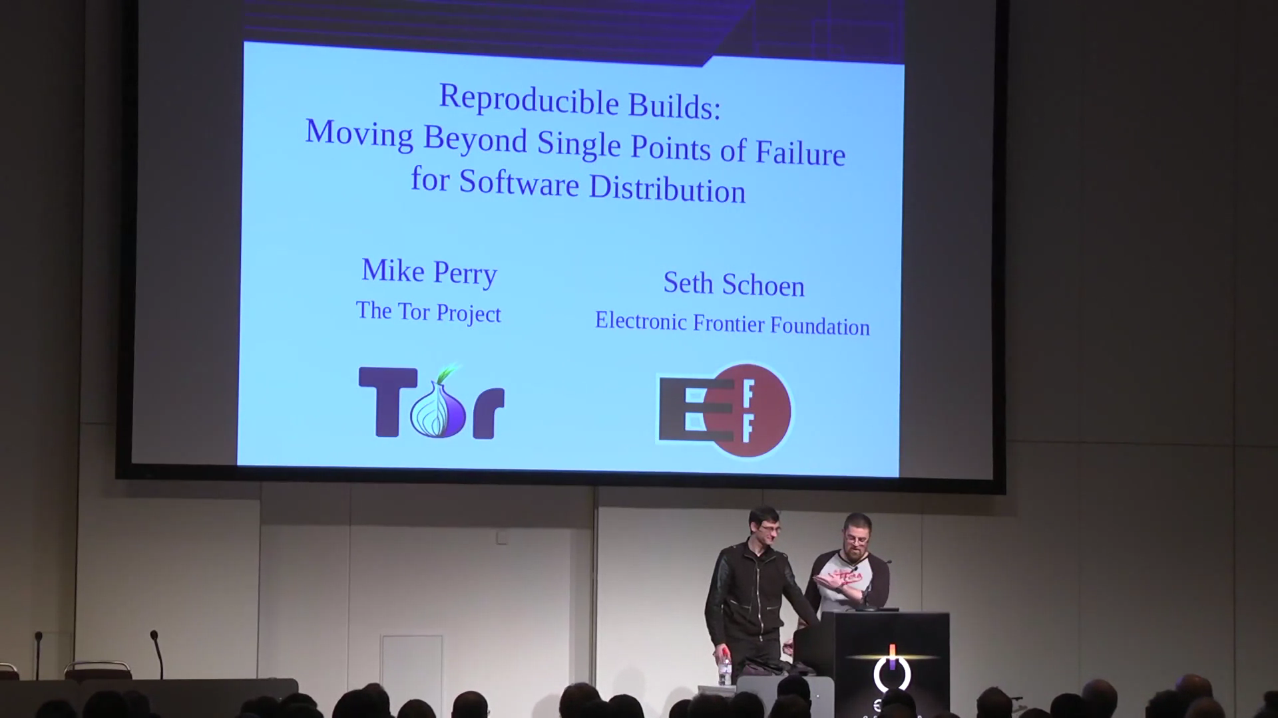
\includegraphics[width=0.7\textwidth]{images/31c3.png}

Available on \url{media.ccc.de}, 31c3
\end{center}

\end{frame}

\begin{frame}[fragile]
\frametitle{Just one example}

At a CIA conference in 2012:

\begin{center}

\includegraphics[width=0.8\textwidth]{images/strawhorse.png}

{\footnotesize 
\url{firstlook.org/theintercept/2015/03/10/ispy-cia-campaign-steal-apples-secrets/}
}
\end{center}

\end{frame}

\begin{frame}
\frametitle{The solution}

\begin{center}
\Large
enable anyone to reproduce\\
identical binary packages\\
from a given source
\end{center}

\end{frame}

\begin{frame}
\frametitle{The solution}

\begin{center}
We call this:

\Huge
“reproducible builds”
\end{center}

\end{frame}

\begin{frame}
\frametitle{It's trendy!}

\begin{itemize}
\item Bitcoin (\textbf{done})
\item Tor (\textbf{done})
\item Debian (\emph{in progress})
\item FreeBSD (\emph{in progress})
\item Coreboot (\textbf{done})
\item OpenWrt (\emph{in progress})
\item \ldots{}
\end{itemize}

\end{frame}

\begin{frame}[plain]
\begin{center}
\Huge It should become the \textbf{norm}.
\end{center}
\end{frame}

\begin{frame}
\frametitle{Multiple aspects}

\begin{itemize}
\item Deterministic build system \\
  \textit{\small for those who write source code}
\item Reproducible build environment \\
  \textit{\small for those who create binaries for others}
\item Distributing the build environment \\
  \textit{\small for those who distribute binaries to the world}
\end{itemize}

\end{frame}

\section{Deterministic build system}

\begin{frame}
\frametitle{Deterministic build system}

In a nutshell:

\begin{itemize}
\item Stable inputs
\item Stable outputs
\item Capture as little as possible from the environment
\end{itemize}
\end{frame}

\begin{frame}[plain]
 \begin{tikzpicture}[remember picture,overlay]
  \node[at=(current page.center)] {
    
\includegraphics[width=\paperwidth]{images/why_is_gone.png}
  };
 \end{tikzpicture}
\end{frame}

\begin{frame}[fragile]
\frametitle{Volatile inputs can disappear}

\begin{itemize}
\item Don't rely on the network
\item If you do, have a backup
\item The binary distributor should provide a fallback
\end{itemize}

\begin{block}{\small FreeBSD does it right}\footnotesize
\begin{semiverbatim}
\$ grep MASTER\_SITES Makefile
MASTER\_SITES= http://gondor.apana.org.au/~herbert/dash/files/
\$ cat distinfo
SHA256 (dash-0.5.8.tar.gz) = c6db3a237747b02d20382a761397563d813b306c020ae28ce25…
SIZE (dash-0.5.8.tar.gz) = 223028
\$ wget http://distcache.freebsd.org/ports-distfiles/distfiles/dash-0.5.8.tar.gz
\end{semiverbatim}
\end{block}
\end{frame}

\begin{frame}[plain]
 \begin{tikzpicture}[remember picture,overlay]
  \node[at=(current page.center)] {
    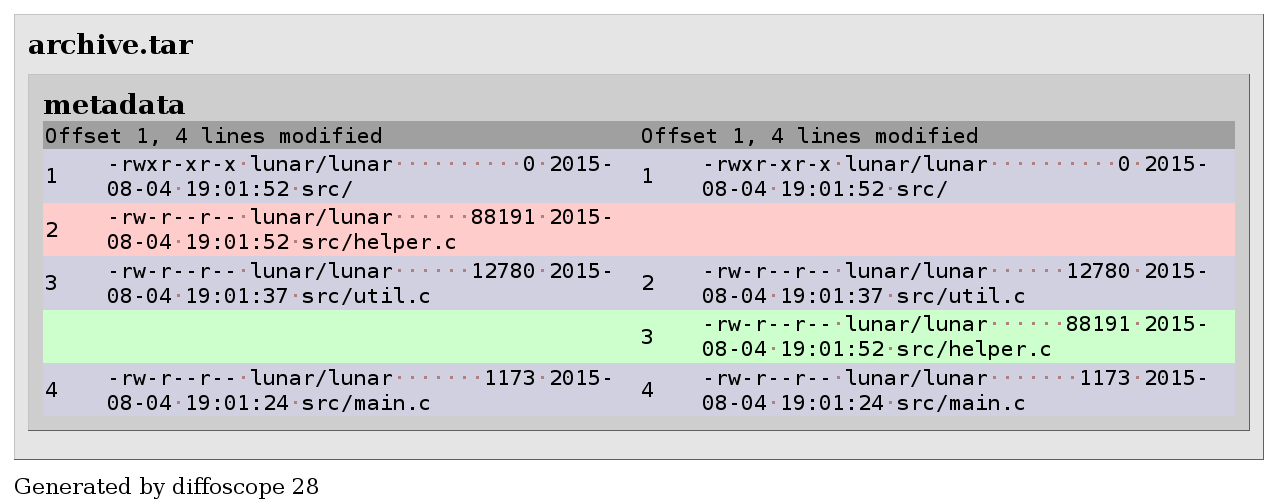
\includegraphics[width=\paperwidth]{images/filesystem_order_in_tarball.png}
  };
 \end{tikzpicture}
\end{frame}

\begin{frame}[fragile]
 \frametitle{Stable order for inputs}

 \begin{itemize}
  \item Always process multiple inputs in the same order
  \item Directory listings are not stable!
  \item<2-> Solutions:
   \begin{itemize}
    \item List inputs explicitely
    \item<3-> Use sorting
    \item<4> \alert{But watch out for difference between locales.}
   \end{itemize}
 \end{itemize}

 \begin{example}
  \begin{overprint}
   \onslide<1>
\begin{semiverbatim}
tar -cf archive.tar src
\end{semiverbatim}
   \onslide<2>
\begin{semiverbatim}
tar -cf archive.tar \\
  src/util.c src/helper.c src/main.c
\end{semiverbatim}
   \onslide<3->
\begin{semiverbatim}
find src -print0 | \only<4>{\alert{LC\_ALL=C} }sort -z |
  tar --null -T - --no-recursion -cf archive.tar
\end{semiverbatim}
  \end{overprint}
 \end{example}
\end{frame}

\begin{frame}[plain]
 \begin{tikzpicture}[remember picture,overlay]
  \node[at=(current page.center)] {
    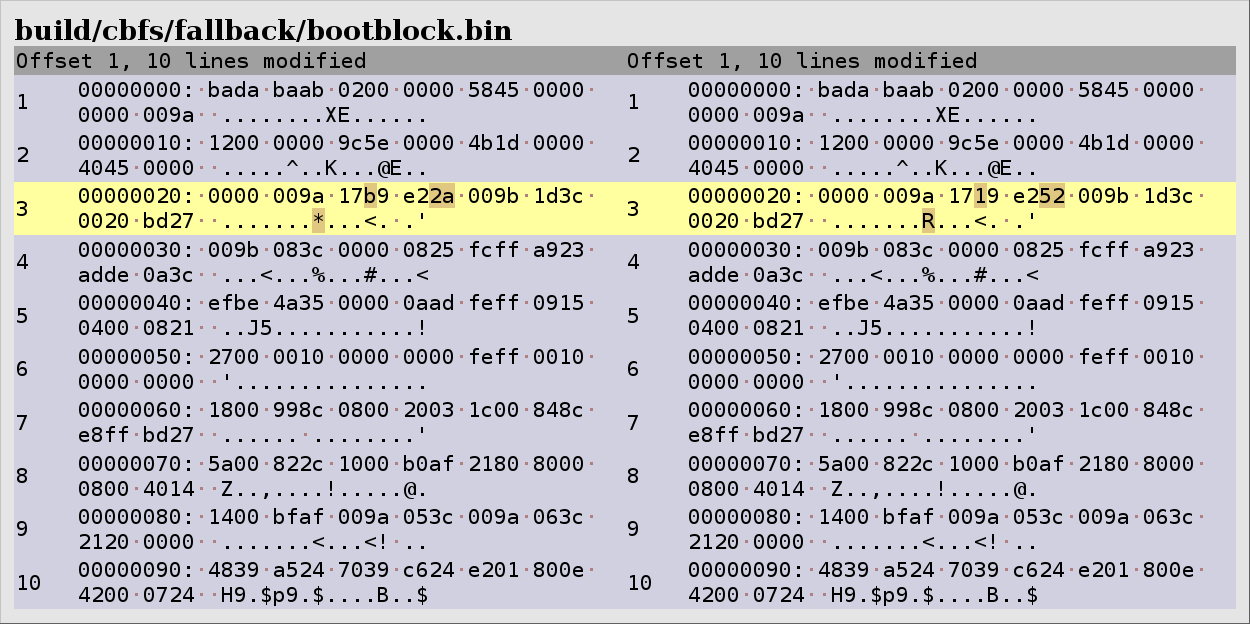
\includegraphics[width=\paperwidth]{images/uninitialized_memory.png}
  };
 \end{tikzpicture}
\end{frame}

\begin{frame}[fragile]
 \frametitle{Controlled value initialization}

 \begin{itemize}
  \item Don't record memory by accident
  \item<2>Always initialize to a known value
 \end{itemize}

 \begin{example}
\begin{semiverbatim}\small
static int write_binary(FILE *out, FILE *in, struct bimg_header *hdr)
\{
       static uint8_t file_buf[MAX_RECORD_BYTES];
       struct bimg_data_header data_hdr\only<2>{\alert{ = \{ 0 \}}};
       size_t n_written;

       data_hdr.dest_addr = hdr->entry_addr;
       …
\end{semiverbatim}
 \end{example}
\end{frame}

\begin{frame}[plain]
 \begin{tikzpicture}[remember picture,overlay]
  \node[at=(current page.center)] {
    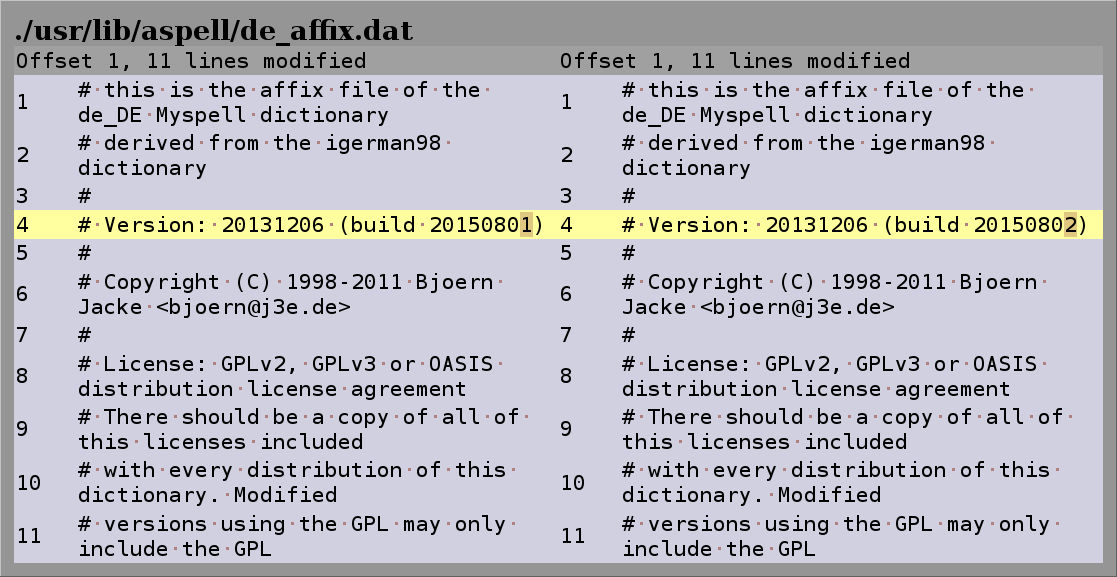
\includegraphics[width=\paperwidth]{images/varying_version.png}
  };
 \end{tikzpicture}
\end{frame}

\begin{frame}[fragile]
 \frametitle{Use deterministic version information}

 \begin{itemize}
  \item Don't make a version number on each build
  \item<2> Instead extract information from the source:
    \begin{itemize}
      \item Version control system revision
      \item Hash of the source code
      \item Changelog entry
    \end{itemize}
 \end{itemize}

 \begin{example}<2>\small
\begin{semiverbatim}
\alert{VERSION=$(shell dpkg-parsechangelog | sed -n 's/^Version: *//p')}

SCONSOPTS = $(SCONSFLAGS) \alert{VERSION=$(VERSION)} \\
  PREFIX=$(PREFIX) PREFIX_CONF=$(SYSCONF) CHMDOCS=0 \\
  STRIP_CP=no \\
  $(if $(findstring nostripfull,$(DEB_BUILD_OPTIONS)),STRIP_W32=no,)
\end{semiverbatim}
 \end{example}
\end{frame}

\begin{frame}[plain]
 \begin{tikzpicture}[remember picture,overlay]
  \node[at=(current page.center)] {
    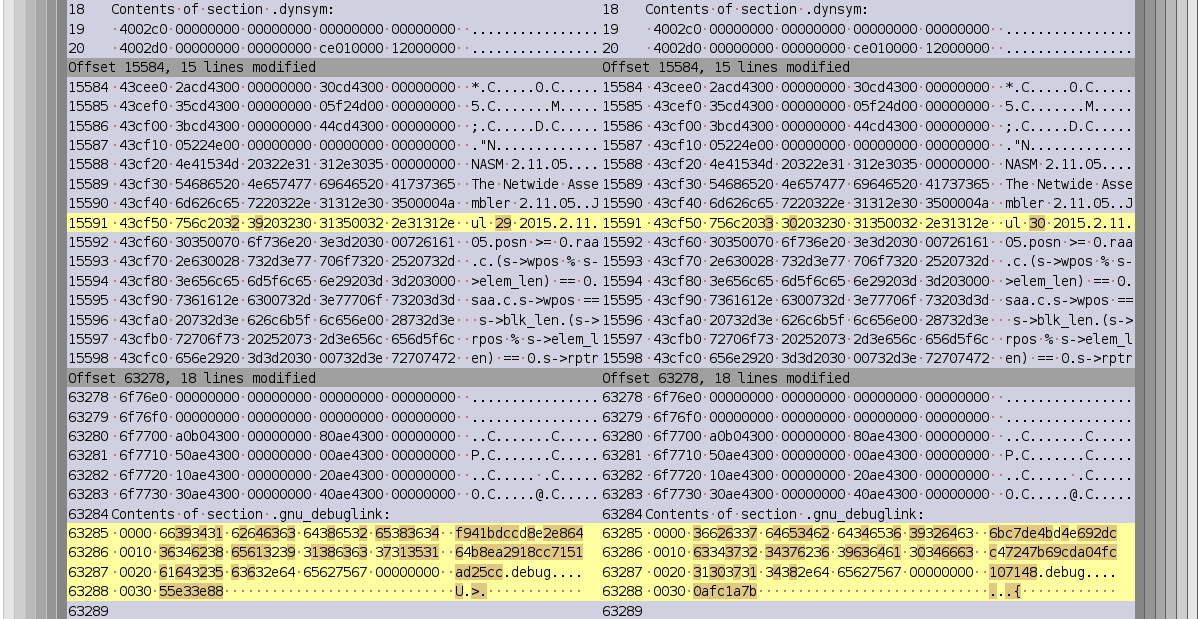
\includegraphics[width=\paperwidth]{images/timestamp_in_nasm.png}
  };
 \end{tikzpicture}
\end{frame}

\begin{frame}
 \frametitle{Don't record the current date and time}

 \begin{itemize}
  \item Avoid timestamps
  \item<2-> If you need one:
    \begin{itemize}
      \item Use date of last commit in VCS
      \item Extract from changelog
      \item<3-> \alert{Don't forget the timezone}
    \end{itemize}
  \item<4-> \texttt{faketime} is an option but has serious drawbacks \\
    {\small \url{https://bugs.torproject.org/12240}}
  \item<5> Implement \texttt{SOURCE\_DATE\_EPOCH}
 \end{itemize}
\end{frame}

\begin{frame}
 \frametitle{SOURCE\_DATE\_EPOCH}

 \begin{itemize}
   \item What is it?
     \begin{itemize}
       \item Environment variable with a reference time
       \item Number of seconds since the Epoch (1970-01-01 00:00:00 +0000 UTC)
       \item If set, replace “current time of day”
       \item Already implemented by \texttt{help2man}, Epydoc, Ghostscript (in Debian)
       \item Patches ready for Doxygen, GCC, \texttt{txt2man}, \texttt{libxslt}, Gettext…
     \end{itemize}
   \item Set it in your build system
   \item Implement it if your tool write timestamps
 \end{itemize}

 \begin{center}
   {\small \url{https://wiki.debian.org/ReproducibleBuilds/TimestampsProposal}}
 \end{center}
\end{frame}

\begin{frame}[plain]
 \begin{tikzpicture}[remember picture,overlay]
  \node[at=(current page.center)] {
    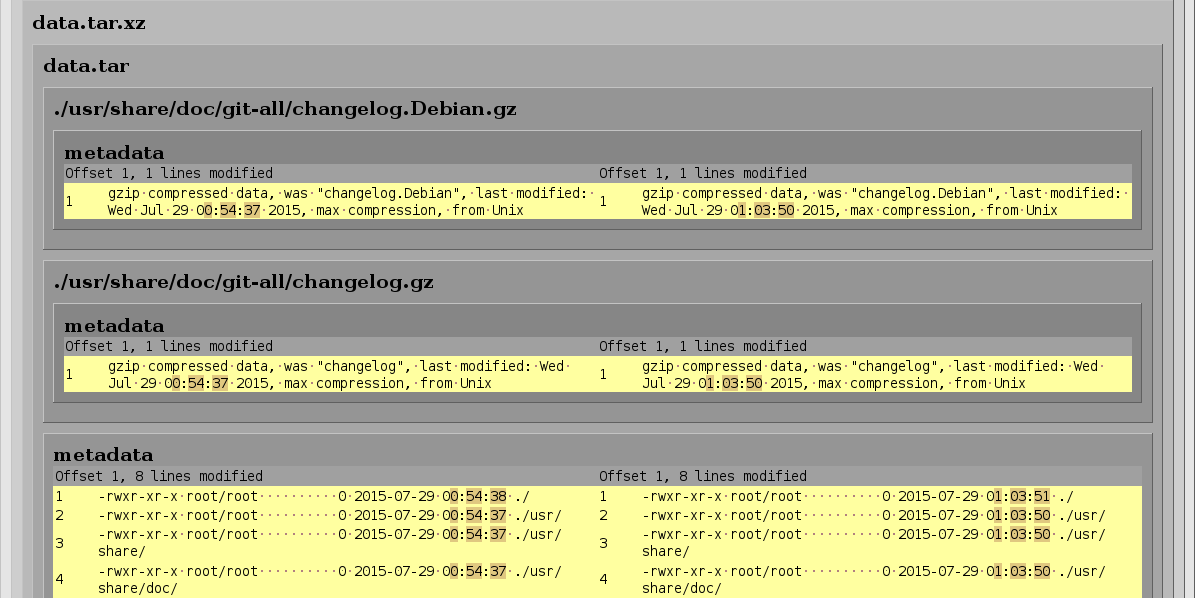
\includegraphics[width=\paperwidth]{images/timestamp_in_git_deb.png}
  };
 \end{tikzpicture}
\end{frame}

\begin{frame}[fragile]
 \frametitle{Don't record current time (really)}

 \begin{itemize}
  \item Archives keep modification times in metadata
  \item Storing a file can record build time
  \item<2-> Solutions:
   \begin{itemize}
    \item Store an arbitrary value
    \item<3-> Pre-process file modification time
    \item<4> Post-process archive
   \end{itemize}
 \end{itemize}

 \begin{example}
\begin{semiverbatim}
\only<1-3>{\visible<3>{\alert{touch --date="2015-08-13 00:00Z" build/*}}
tar\only<2>{\alert{ --mtime='2015-08-13 00:00Z'}} -cf product.tar build
}\only<4>{\textit{\color[rgb]{.7,.7,.7}# zip has no equivalent of --mtime}
zip product.zip build
\alert{strip-nondeterminism product.zip}}
\end{semiverbatim}
 \end{example}
\end{frame}

\begin{frame}[plain]
 \begin{tikzpicture}[remember picture,overlay]
  \node[at=(current page.center)] {
    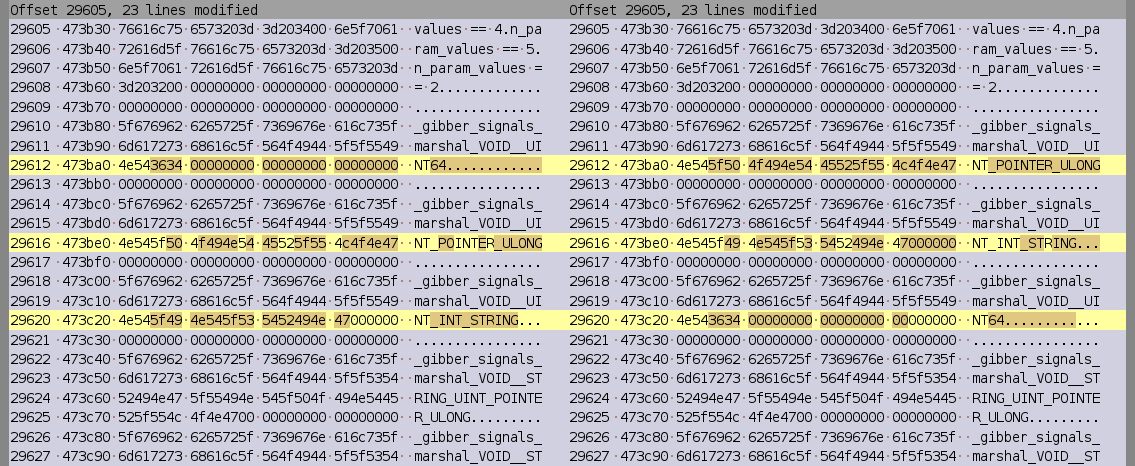
\includegraphics[width=\paperwidth]{images/random_function_order.png}
  };
 \end{tikzpicture}
\end{frame}

\begin{frame}[fragile]
 \frametitle{Stable order for outputs}

 \begin{itemize}
  \item Always output lists in the same order
  \item Typical issue: key order with hash tables
  \item<2> Sort!
 \end{itemize}

 \begin{example}
\begin{semiverbatim}
for module in \only<2>{\alert{sorted(}}dependencies.keys()\only<2>{\alert{)}}:
    version = dependencies[module]
    print('\%s (>= \%s)' \% (module, version))
\end{semiverbatim}
 \end{example}
\end{frame}

{
\usebackgroundtemplate{%
 \begin{tikzpicture}[remember picture,overlay]%
  \node[shift={(-0.2\paperwidth, -0.2\paperheight)},at=(current page.north east)] {
    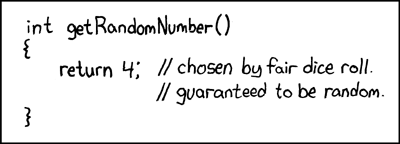
\includegraphics[width=0.3\paperwidth]{images/random_number.png}
  };
 \end{tikzpicture}%
}
\begin{frame}[fragile]
 \frametitle{Avoid (true) randomness}

 \begin{itemize}
  \item Randomness is not deterministic
  \item<2-> Seed for your PRNG from known value
   \begin{itemize}
     \item Use a fixed value
     \item<3> Extract from source code (filename, content hash)
   \end{itemize}
 \end{itemize}

 \begin{example}
\begin{semiverbatim}\small
\$ gcc -c\only<2->{ \alert{-frandom-seed=}}\only<2>{\alert{0}}\only<3>{\alert{utils.o}} utils.c
\$ nm -a utils.o | grep inline
\only<1>{0000000000000000 n .gnu.lto\_.inline.381a277a0b6d2a35}\only<2>{0000000000000000 n .gnu.lto\_.inline.0}\only<3>{0000000000000000 n .gnu.lto\_.inline.a108e942}
\end{semiverbatim}
 \end{example}
\end{frame}
}

\begin{frame}
 \frametitle{Define environment variable affecting outputs}

 \begin{itemize}
  \item Some environment variables will affect software outputs. E.g:
   \begin{itemize}
    \item \texttt{LC\_CTIME} for time strings
    \item \texttt{LC\_CTYPE} for text encoding
    \item \texttt{TZ} for times
   \end{itemize}
  \item<2-> Set them to a controlled value
  \item<3> \textit{Please don't force the language}
 \end{itemize}
\end{frame}

\begin{frame}
 \frametitle{Stop recording build system information}

 \begin{itemize}
  \item Don't record information about the build system, like:
   \begin{itemize}
    \item date and time of the build
    \item hostname
    \item path
    \item network configuration
    \item CPU
    \item environment variables
    \item …
   \end{itemize}
  \item<2> If you really want to record them, do it outside the binaries
 \end{itemize}
\end{frame}

\section{Reproducible build environment}

\begin{frame}
 \frametitle{What's in a build environment?}

 \begin{itemize}
  \item At least: build tools and their specific versions
  \item Up to you, depending on the build system:
   \begin{itemize}
    \item build architecture
    \item kernel
    \item \textit{build path}
    \item \textit{build date and time}
    \item …
   \end{itemize}
 \end{itemize}
\end{frame}

\begin{frame}
 \frametitle{Build from source}

 \begin{itemize}
  \item Build tools affecting the output from source
  \item Record version / tag / git commit
  \item Approach used by Coreboot, OpenWrt, \textit{Tor Browser}
 \end{itemize}
\end{frame}

\begin{frame}
 \frametitle{Reference distribution}

 \begin{itemize}
  \item Use a stable distribution (e.g. Debian, CentOS)
  \item Record package version
  \item Hope the old package will stay available / record
  \item Approach used by Bitcoin
 \end{itemize}
\end{frame}

\begin{frame}
 \frametitle{Virtual machines / containers}

 \begin{itemize}
  \item Using a VM saves some problems:
   \begin{itemize}
    \item Same user
    \item Same hostname
    \item Same network configuration
    \item \textit{Same CPU}
    \item …
   \end{itemize}
  \item Introduce new things that needs to be trusted
 \end{itemize}
\end{frame}

\begin{frame}
 \frametitle{Proprietary operating systems}

 \begin{itemize}
  \item Cross-compiling to the rescue!
  \item For Windows:
   \begin{itemize}
     \item mingw-w64: build Windows binaries on *nix
     \item NSIS (Nullsoft Scriptable Install System)
   \end{itemize}
  \item For Mac OS X:
   \begin{itemize}
     \item Hackish, but doable \\
       {\footnotesize \url{https://github.com/bitcoin/bitcoin/blob/master/doc/README\_osx.txt}}
     \item Recent versions of clang for compiling
     \item Patched \texttt{cctools} (linker, etc.)
     \item Non-redistributable SDK extracted from XCode
     \item \texttt{.dmg} are a bit tricky
   \end{itemize}
 \end{itemize}
\end{frame}

\section{Distributing the build environment}

\begin{frame}
 \frametitle{Good ol'Makefile}

 \begin{itemize}
  \item Download known toolchain archive
  \item Compare reference checksums
  \item Build and setup
  \item Coreboot: \texttt{make crossgcc}
 \end{itemize}
\end{frame}

\begin{frame}
 \frametitle{Check-in everything}

 \begin{itemize}
  \item Check-in all the toolchain source code in VCS
  \item Approach used for the base system in *BSD, and Google
  \item Make sure everything is checked in (\textit{use sandbox on Linux})
  \item Recently open-sourced: Bazel \\
   \url{http://bazel.io/}
  \item Can be hard to ask everyone to download everything all the time
 \end{itemize}
\end{frame}

\begin{frame}[fragile]
 \frametitle{Ship the toolchain as a build product}

 \begin{itemize}
  \item Make the toolchain as a build product
  \item OpenWrt:
    \url{http://wiki.openwrt.org/doc/howto/obtain.firmware.sdk}
 \end{itemize}

 \begin{example}\footnotesize
\begin{semiverbatim}
\$ wget https://downloads.openwrt.org/…/14.07/…OpenWrt-SDK-atheros-….tar.bz2
\$ svn export svn://…/branches/packages\_14.07/utils/xz package/xz
\$ make package/xz/compile
\end{semiverbatim}
 \end{example}

\end{frame}

\begin{frame}
 \frametitle{Gitian}

 \begin{itemize}
  \item Used by Bitcoin, Tor Browser
  \item Drives LXC or KVM
  \item “Descriptors” describing the build using:
   \begin{itemize}
    \item Base distribution
    \item Packages
    \item Git remotes
    \item Other input files
    \item Build script
   \end{itemize}
 \end{itemize}

 \vfill
 \begin{block}{\footnotesize Resources}\footnotesize
 \url{https://gitian.org/}\\
 \url{https://github.com/bitcoin/bitcoin/blob/master/doc/gitian-building.md}\\
 \url{https://github.com/bitcoin/bitcoin/blob/master/contrib/gitian-descriptors/}
 \end{block}
\end{frame}

\begin{frame}[fragile]
 \frametitle{Docker}

 \begin{itemize}
  \item Provide a way to describe specialized Linux container images
  \item Build in a controlled environment
  \item Docker image can be addressed with a hash of their content
  \item Bazel has support to build Docker image reproducibly
 \end{itemize}

 \begin{block}{\footnotesize \url{https://github.com/tianon/gosu/blob/master/Dockerfile}}\footnotesize
\begin{semiverbatim}
FROM golang:1.4-cross
[…]
# disable CGO for ALL THE THINGS (to help ensure no libc)
ENV CGO\_ENABLED 0
COPY *.go /go/src/github.com/tianon/gosu/
WORKDIR /go/src/github.com/tianon/gosu
RUN GOARCH=amd64 go build -v -ldflags -d -o /go/bin/gosu-amd64
\end{semiverbatim}
 \end{block}
\end{frame}

\begin{frame}
 \frametitle{Vagrant}

 \begin{itemize}
  \item Drive VirtualBox using Ruby and other scripts
  \item Build in a controlled environment
  \item Also works under OS X and Windows
 \end{itemize}

 \vfill
 {\footnotesize
 \url{https://www.vagrantup.com/}
 }
\end{frame}

\begin{frame}
 \frametitle{Debian .buildinfo}

 \begin{itemize}
  \item Tie in the same file:
   \begin{itemize}
    \item Sources
    \item Generated binaries
    \item Packages used to build (with specific version)
   \end{itemize}
  \item Can be later processed to reinstall environment
  \item All versions are available from \url{snapshot.debian.org}
 \end{itemize}
\end{frame}

\begin{frame}[fragile]
 \frametitle{Example .buildinfo}

{\small
\begin{verbatim}
Format: 1.9
Build-Architecture: amd64
Source: txtorcon
Binary: python-txtorcon
Architecture: all
Version: 0.11.0-1
Build-Path: /usr/src/debian/txtorcon-0.11.0-1
Checksums-Sha256:
 a26549d9…7b 125910 python-txtorcon_0.11.0-1_all.deb
 28f6bcbe…69 2039 txtorcon_0.11.0-1.dsc
Build-Environment:
 base-files (= 8),
 base-passwd (= 3.5.37),
 bash (= 4.3-11+b1),
 …
\end{verbatim}
}
\end{frame}

\section{Tips}

\begin{frame}
 \frametitle{Testing for variations}

 \begin{itemize}
  \item Build a first time
  \item Save the result
  \item Perform change to the environment
  \item Build a second time
  \item Compare results
 \end{itemize}
\end{frame}

\begin{frame}
 \frametitle{reproducible.debian.net}

 \begin{itemize}
  \item Continuous test system driven by Jenkins
  \item Bad ass hardware sponsored by ProfitBricks
  \item Tests about 1300 Debian source packages per day on average
  \item Results are visible on a website
  \item Other projects: Coreboot, OpenWrt, \textit{yours?}
 \end{itemize}
 \vfill
 \begin{center}
 
\includegraphics[height=0.15\paperheight]{images/profitbricks_logo.png}
 \end{center}
\end{frame}

\begin{frame}[fragile]
 \frametitle{Variations on reproducible.debian.net}

 \begin{center}
  \begin{table}
   \resizebox{0.95\textwidth}{!}{%
    \begin{tabular}{l|ll}
\textbf{variation} & \textbf{first build} & \textbf{second build} \\
\hline
hostname & \texttt{jenkins} & \texttt{i-capture-the-hostname} \\
domainname & \texttt{debian.net} & \texttt{i-capture-the-domainname} \\
\texttt{env TZ} & \texttt{GMT+12} & \texttt{GMT-14} \\
\texttt{env LANG} & \texttt{en\_GB.UTF-8} & \texttt{fr\_CH.UTF-8} \\
\texttt{env LC\_ALL} & not set & \texttt{fr\_CH.UTF-8} \\
\texttt{env USER} & \texttt{pbuilder1} & \texttt{pbuilder2} \\
uid & \texttt{1111} & \texttt{2222} \\
gid & \texttt{1111} & \texttt{2222} \\
UTS namespace & shared with the host & \textit{modified using \texttt{/usr/bin/unshare --uts}} \\
kernel version & Linux 3.16.0-4-amd64 & Linux 2.6.56-4-amd64 \\
umask & 0022 & 0002 \\
CPU type & \multicolumn{2}{l}{same for both builds \textit{(work in progress)}} \\
year, month, date & \multicolumn{2}{l}{same for both builds \textit{(work in progress)}} \\
hour, minute & \multicolumn{2}{l}{hour is usually the same… usually, the minute differs… \textit{(work in progress)}} \\
\textit{everything else} & \multicolumn{2}{l}{\textit{is likely the same…}}
    \end{tabular}
   }
  \end{table}
 \end{center}
\end{frame}

{
\usebackgroundtemplate{%
 \begin{tikzpicture}[remember picture,overlay]%
  \node[shift={(-0.15\paperwidth, 0.4\paperheight)},at=(current page.south east)] {
    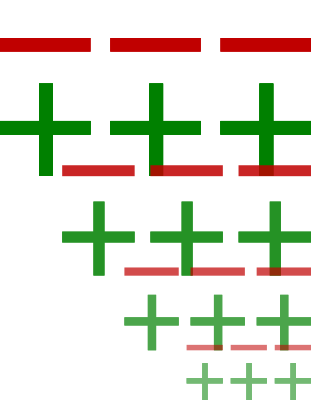
\includegraphics[width=0.2\paperwidth]{images/diffoscope_logo.png}
  };
 \end{tikzpicture}%
}
\begin{frame}{diffoscope}
 \frametitle{Debbuging problems: diffoscope}

 \begin{itemize}
  \item Examines differences \textbf{in depth}
  \item Outputs HTML or plain text showing the differences
  \item Recursively unpack archives
  \item Seeks human readability:
   \begin{itemize}
    \item uncompress PDF
    \item disassemble binaries
    \item unpack Gettext files
    \item … \textit{easy to extend to new file formats}
   \end{itemize}
  \item Falls back to binary comparison
 \end{itemize}
 \vfill
 \begin{center}
  \url{http://diffoscope.org/}
 \end{center}
\end{frame}
}

\begin{frame}
 \frametitle{diffoscope example (HTML output)}

 \begin{center}
  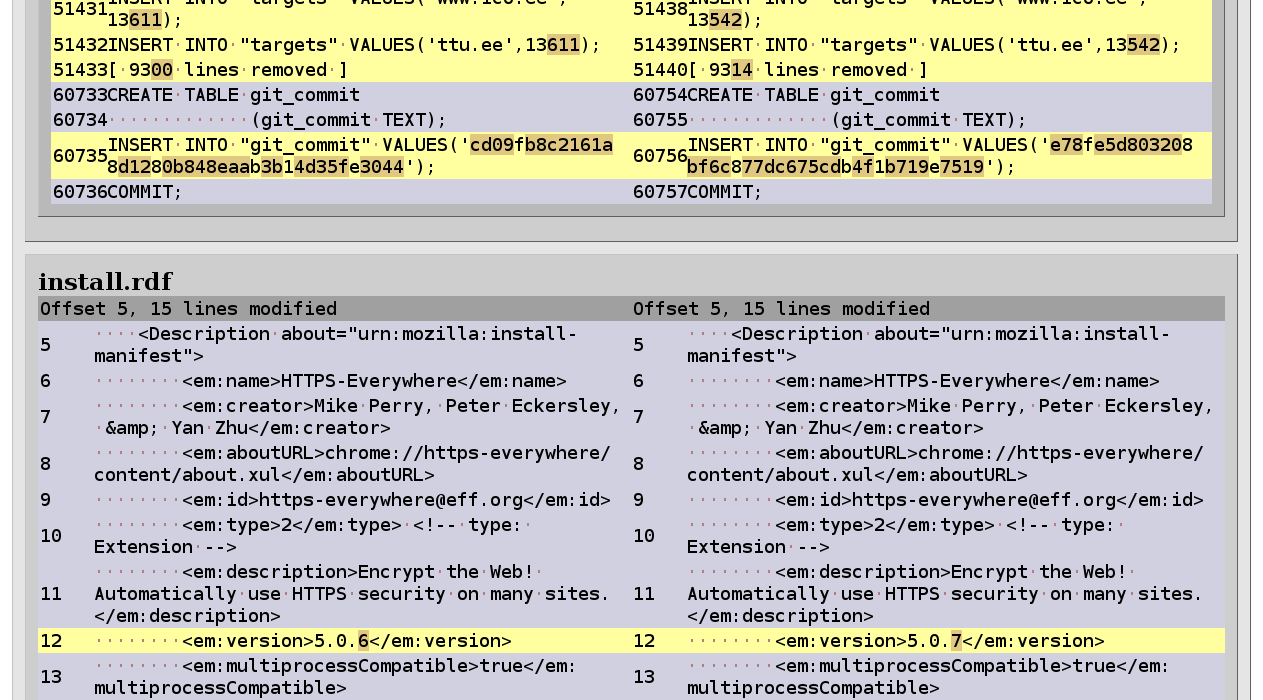
\includegraphics[width=0.9\paperwidth]{images/diffoscope_example_html.png}
 \end{center}
\end{frame}

\begin{frame}
 \frametitle{diffoscope example (text output)}

 \begin{center}
  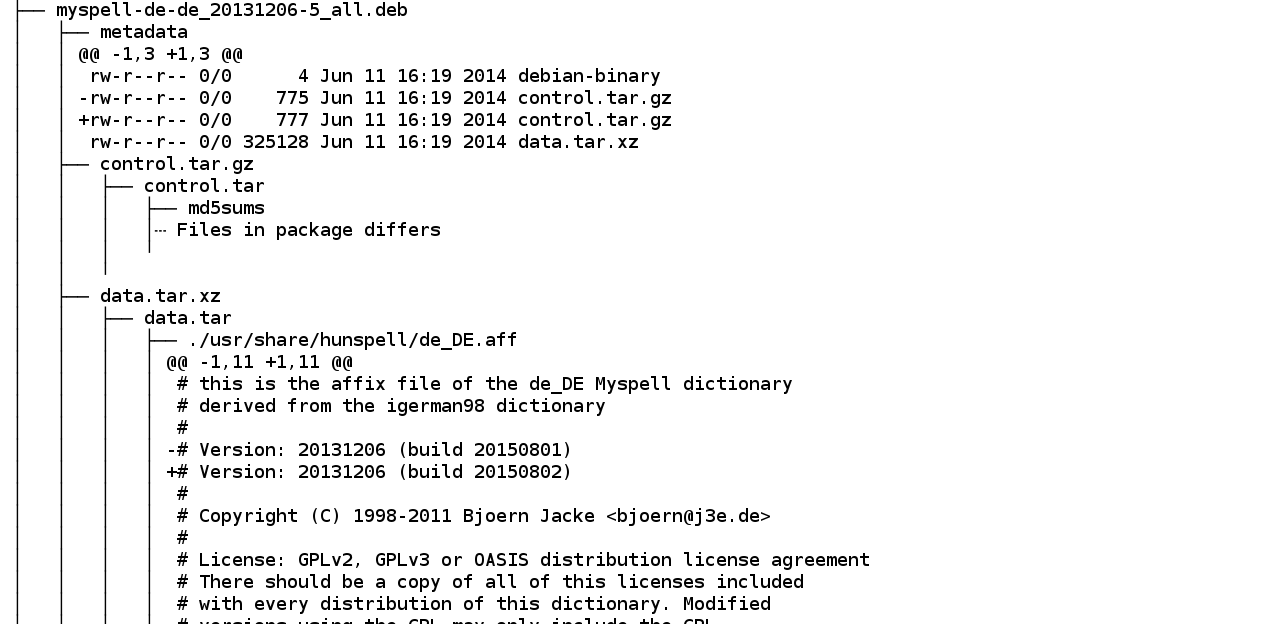
\includegraphics[width=0.9\paperwidth]{images/diffoscope_example_text.png}
 \end{center}
\end{frame}

\begin{frame}
 \frametitle{strip-nondeterminism}

 \begin{itemize}
  \item Normalize various file formats
  \item Currently handles:
   \begin{itemize}
    \item ar archives (\texttt{.a})
    \item gzip
    \item Java jar
    \item Javadoc HTML
    \item Maven \texttt{pom.properties}
    \item PNG
    \item ZIP archives
    \item … \textit{extensible to new formats}
   \end{itemize}
  \item Written in Perl (like \texttt{dpkg-dev})
 \end{itemize}
\end{frame}

\begin{frame}
 \frametitle{Resources}

 \begin{itemize}
  \item Reproducible Builds HOWTO (\textit{work in progress})\\
   \url{https://reproducible.debian.net/howto/}
  \item Debian “Reproducible Builds” wiki \\
   \url{https://wiki.debian.org/ReproducibleBuilds}
  \item Diverse Double-Compilation \\
   \url{http://www.dwheeler.com/trusting-trust/}
 \end{itemize}
\end{frame}

\section{Question?}

\begin{frame}
 \frametitle{Thanks!}

 \begin{itemize}
  \item Debian “Reproducible Builds” team \\
    {\small (you are just \textbf{so} awesome!)}
  \item Mike Perry, Georg Koppen, David A. Wheeler
  \item Linux Foundation and the Core Infrastructure Initiative
 \end{itemize}

 \begin{center}
  
\includegraphics[height=0.1\paperheight]{images/linux_foundation_logo.png}
  \hspace{0.1\paperwidth}
  
\includegraphics[height=0.1\paperheight]{images/cii_logo.png}
 \end{center}

 \vfill
 \begin{center}
  \begin{tabular}{rl}
   \texttt{lunar@debian.org} & \texttt{0603 CCFD 9186 5C17 E88D} \\
                             & \texttt{4C79 8382 C95C 2902 3DF9}
  \end{tabular}
 \vfill
 \begin{center}\footnotesize
  clothes: Elhonna Sombrefeuille — hair: igor
 \end{center}

 \end{center}
\end{frame}

\end{document}
